\documentclass{beamer}
\usepackage{handout}
\title{PS-1006: Politics - Preliminary}
\author{Tom T. Hsiao}
\date{\today}
\begin{document}
\fontspec{Times New Roman}
\begin{frame}
\begin{center}
\Large{Lesson 0 Preliminary} \\
\vspace{3em}
\normalsize{Instructor: Tzu-Chi Hsiao} \\
\vspace{3em}
\small{Department of Political Science} \\
\vspace{1em}
\small{University} \\
\end{center}
\end{frame}
\begin{frame}{}
\begin{center}

\includegraphics[width=0.35\textwidth]{instructor.png}
\end{center}
\vspace{1em}
\begin{center}
\large{Welcome to enroll Politics !} \\
\end{center}
\end{frame}
\begin{frame}{Mutual Encouragement}
\begin{center}

\includegraphics[width=0.35\textwidth]{mc.png}
\end{center}
\begin{center}
Unity of knowledge and action.
\end{center}
\flushright Yang-Ming Wang
\end{frame}
\begin{frame}{Angel or Demon}
\begin{minipage}{0.45\textwidth}
\begin{center}

\includegraphics[width=0.7\textwidth]{heal.png}
\end{center}
\begin{center}
May be an angel in your grade.
\end{center}
\end{minipage}
\hfill
\begin{minipage}{0.45\textwidth}
\begin{center}

\includegraphics[width=0.7\textwidth]{kill.png}
\end{center}
\begin{center}
May be a demon during the examination.
\end{center}
\end{minipage}
\end{frame}
\begin{frame}{Except myself}
\begin{center}
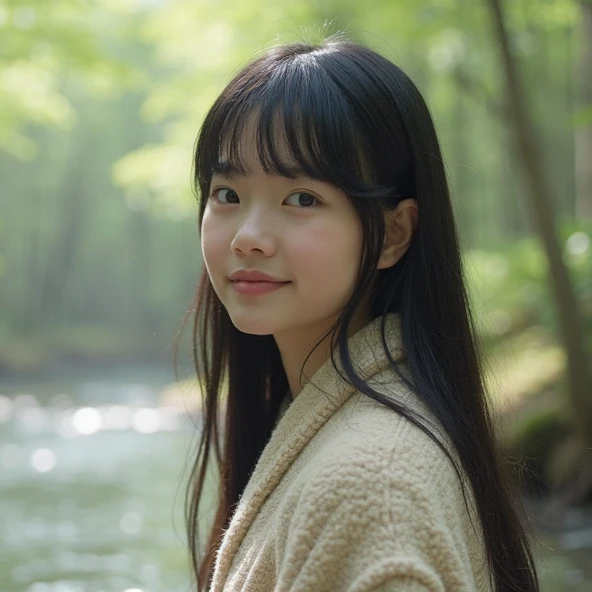
\includegraphics[width=0.35\textwidth]{tchsiao.png}
\end{center}
\begin{center}
Interesting instructor and grading equality.
\end{center}
\end{frame}
\begin{frame}{Why taking this course}
\begin{itemize}
\item Politics happens \textcolor{red}{everywhere and everyday}.
\item We interest in process and results.
\end{itemize}
\end{frame}
\begin{frame}{Course Grading}
\begin{center}
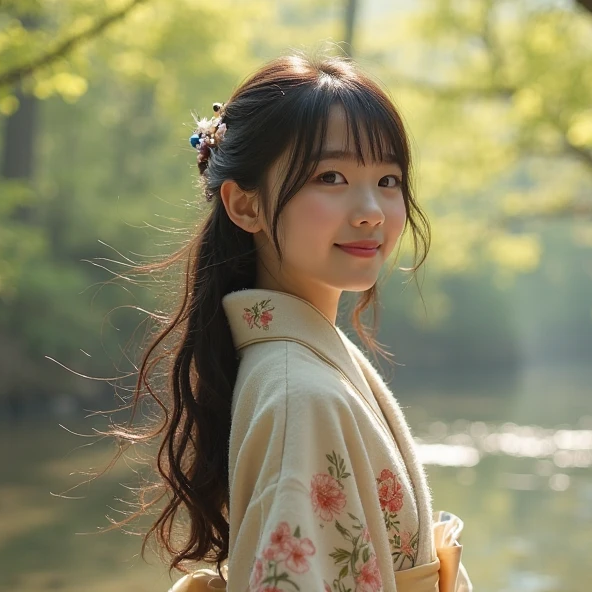
\includegraphics[width=0.35\textwidth]{examination.png}
\end{center}
\begin{center}
Final 100\% with \textcolor{red}{AEP}.
\end{center}
\end{frame}
\begin{frame}{Course Grading (Cont'd)}
Forms of examinations:
\begin{itemize}
\item Short essay: 100\%, separate as 35\%, 35\%, 30\% each.
\item You can take a textbook or unlimited A4 double sided note to answer our problems.
\end{itemize}
\end{frame}
\begin{frame}{Adjusting overall score}
\setbeamercolor{block title}{bg=red, fg=white}
\setbeamercolor{item}{fg=red}
\begin{block}{Description}
\begin{itemize}
\item The overall score adjust by the instructor to achieve the Average Equility Policy (AEP).
\end{itemize}
\end{block}
\setbeamercolor{block title}{bg=orange, fg=white}
\setbeamercolor{item}{fg=orange}
\begin{block}{Average Equility Policy (AEP)}
\begin{itemize}
\item The overall contains who quitted the course.
\item The highest score will be adjusted to 99 points.
\item If there is a saving zone, others may gain one additional point.
\end{itemize}
\end{block}
\end{frame}
\begin{frame}{Course Policy}
\begin{enumerate}
\item Cheating or plagiarism will be dropped out from the course with \textcolor{red}{zero points} and \textcolor{red}{huge demerit}. \\
\end{enumerate}
\end{frame}
\begin{frame}{Sharing time}
\begin{itemize}
\item What do we need to study in University.
\item What do we need to study in Political Science.
\end{itemize}
\end{frame}
\begin{frame}{Sharing time}
\begin{itemize}
\item What do we need to study in University.
\item \textcolor{gray}{What do we need to study in Political Science.}
\end{itemize}
\end{frame}
\begin{frame}{Study in University}
\begin{center}
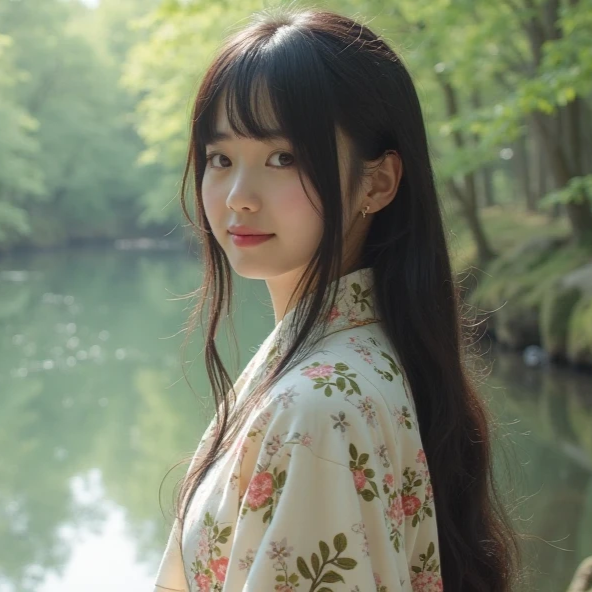
\includegraphics[width=0.35\textwidth]{target.png}
\end{center}
\begin{itemize}
\item \textcolor{red}{Target} is the most important direction within your whole life.
\end{itemize}
\end{frame}
\begin{frame}{Sharing time}
\begin{itemize}
\item \textcolor{gray}{What do we need to study in University.}
\item What do we need to study in Political Science.
\end{itemize}
\end{frame}
\begin{frame}{Study in Political Science}
\begin{center}
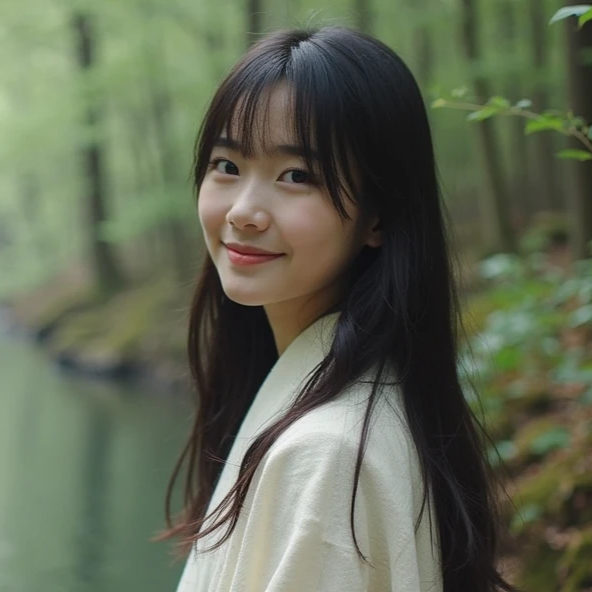
\includegraphics[width=0.35\textwidth]{motivate.png}
\end{center}
\begin{itemize}
\item Political Science seems a \textcolor{red}{jumper} department for those who interested in result.
\end{itemize}
\end{frame}
\begin{frame}{Endeavor or Laid flat}
\begin{center}

\includegraphics[width=0.35\textwidth]{fail.png}
\end{center}
\begin{center}
Endeavor is the key to success, unless you want me to become your friend.
\end{center}
\end{frame}
\begin{frame}{Reason letter}
\begin{center}

\includegraphics[width=0.35\textwidth]{endeavor.png}
\end{center}
\begin{center}
You will receive a reason letter if you fail in the course.
\end{center}
\end{frame}
\begin{frame}{Contact}
\begin{center}

\includegraphics[width=0.35\textwidth]{kg.png}
\end{center}
\begin{center}
Use E-mail to contact me.
\end{center}
\end{frame}
\begin{frame}{}
\begin{center}
\Large{End of Lesson 0}
\end{center}
\end{frame}
\end{document}
